\section{Огляд алгоритмів пошуку маршрутів}
\label{sec:route-search-algorithms}

Пошук маршрутів є критично важливим завданням у плануванні перевезень та логістики. Воно передбачає пошук найефективнішого шляху між двома або більше пунктами на основі різних обмежень, таких як час, відстань, вартість, трафік та інші фактори. Для цього існує кілька алгоритмів і методів, які були розроблені протягом багатьох років для вирішення проблеми пошуку маршрутів.

Одним з найпопулярніших алгоритмів пошуку найкоротшого шляху між двома точками є алгоритм Дейкстри. Цей алгоритм широко використовується в протоколах мережевої маршрутизації та навігаційних системах GPS. Він працює, досліджуючи всі можливі шляхи від вузла-джерела до вузла призначення, відстежуючи шлях з найнижчою вартістю. Однак алгоритм Дейкстри не є ефективним для великомасштабних задач пошуку маршрутів, оскільки він вимагає обробки всіх вершин і ребер графа.

Іншим підходом є алгоритм A*, який є розширенням алгоритму Дейкстри, що використовує евристики для більш ефективного спрямування пошуку до вузла призначення. A* враховує як відстань від вихідного вузла, так і оцінку відстані, що залишилася до вузла призначення, щоб визначити наступний вузол для дослідження. Це робить A* більш ефективним, ніж алгоритм Дейкстри, для великомасштабних задач пошуку маршрутів.

Крім цих алгоритмів, існує ще кілька методів пошуку маршрутів, зокрема алгоритм Беллмана-Форда, алгоритм Флойда-Уоршалла, алгоритм Джонсона та алгоритм пошуку в ширину. Ці алгоритми мають свої сильні та слабкі сторони і підходять для різних типів задач пошуку маршрутів.

Нижче кожен з існуючих алгоритмів буде розглянуто більш детально.

% Subsections
\subsection{Алгоритм Дейкстри}
\label{subsec:dijkstra-subsection}

Алгоритм Дейкстри --- це широко використовуваний алгоритм для пошуку найкоротшого шляху між двома вершинами зваженого графа. Він був винайдений комп'ютерним вченим Едсгером В. Дейкстрою в 1956 році. Алгоритм дуже ефективний для пошуку найкоротшого шляху в графах з невід'ємними вагами ребер.

Основна ідея алгоритму полягає в тому, щоб почати з початкової вершини і відвідати всі вершини, доступні з початкової вершини. Для кожної відвіданої вершини алгоритм оновлює відстані до всіх сусідніх вершин, які ще не були відвідані. Для цього він порівнює відстань від початкової вершини до сусідніх вершин через поточну вершину з раніше обчисленою відстанню до цих вершин. Якщо новообчислена відстань менша, він оновлює відстань і встановлює поточну вершину як новий попередній вузол на шляху до цієї вершини.

Цей процес повторюється до тих пір, поки не будуть відвідані всі вершини, до яких можна дістатися з початкової вершини. Після завершення алгоритм повертає найкоротший шлях від початкової вершини до всіх інших вершин графа.

Однією з головних переваг алгоритму Дейкстри є його простота і легкість реалізації. Він також гарантує знаходження оптимального розв'язку для графа з невід'ємною вагою. Однак він може бути повільним при роботі з великими графами, оскільки йому потрібно оцінити всі вершини і ребра, доступні з вихідної вершини. Крім того, він не працює з від'ємними вагами ребер і може бути не найкращим варіантом для певних типів графів, наприклад, для графів з великою кількістю від'єднаних вершин.

\begin{figure}[!htp]
    \centering
    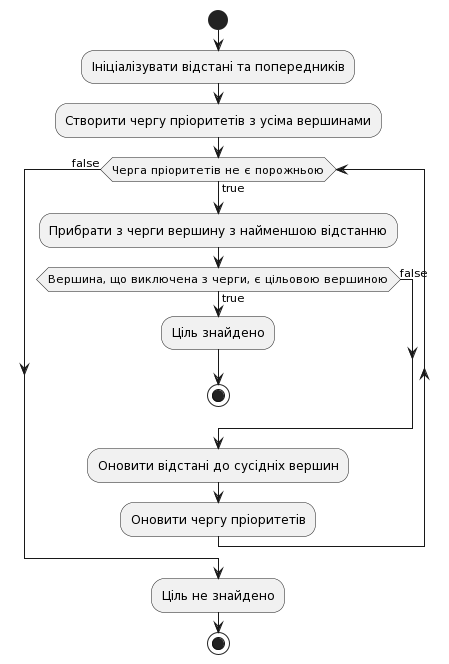
\includegraphics[scale=0.7]{content/chapters/2-implementation-methods/assets/img/dijkstras_algorithm.png}
    \caption{Блок-схема алгоритму Дейкстри}
    \label{fig:dijkstras}
\end{figure}

Переваги:
\begin{itemize}
    \item Гарантує знаходження найкоротшого шляху у зваженому графі з невід'ємними вагами ребер.
    \item Це відносно простий і зрозумілий алгоритм, що робить його гарним вибором для навчальних цілей.
    \item Його можна використовувати в широкому спектрі застосувань, від маршрутизації в комп'ютерних мережах до пошуку найкоротшого шляху в транспортних мережах.
    \item Він може обробляти графи з декількома шляхами однакової ваги, на відміну від деяких інших алгоритмів, які можуть працювати з такими випадками некоректно.
\end{itemize}

Недоліки:
\begin{itemize}
    \item Не працює коректно з від'ємними вагами ребер, оскільки може застрягти у нескінченному циклі.
    \item Може бути повільним на великих графах, особливо якщо черга пріоритетів, яка використовується для реалізації, не є ефективною.
    \item Він може бути не найкращим вибором для певних типів графів, наприклад, графів з високим ступенем зв'язності або графів з великою кількістю циклів.
    \item Він не обробляє графи з декількома найкоротшими шляхами між однією і тією ж парою вершин.
\end{itemize}


\subsection{A*}
\label{subsec:a-star-subsection}

Алгоритм A* --- це широко використовуваний алгоритм пошуку шляху, який є розширенням алгоритму Дейкстри. Як і алгоритм Дейкстри, A* використовує евристичну функцію для спрямування пошуку до цільової вершини, але він також враховує вартість вже пройденого шляху. Це дозволяє йому здійснювати пошук більш ефективно, досліджуючи спочатку найбільш перспективні шляхи.

Алгоритм A* працює, підтримуючи два списки: відкритий і закритий. Відкритий список містить вузли, які були відвідані, але ще не розширені, тоді як закритий список містить вузли, які вже були розширені. Спочатку у відкритому списку знаходиться лише початкова вершина. Потім алгоритм багаторазово вибирає вершину з найменшим значенням f (де f(n) = g(n) + h(n), де g(n) - вартість шляху від початкової вершини до вершини n, а h(n) - евристична оцінка вартості шляху від вершини n до мети) і розширює її, додаючи до відкритого списку її сусідів, якщо вони ще не були відвідані.

Алгоритм A* продовжує роботу до тих пір, поки цільова вершина не буде обрана для розширення або поки відкритий список не стане порожнім (в цьому випадку не буде шляху до цільової вершини). Як тільки цільовий вузол досягнуто, алгоритм відстежує шлях назад, слідуючи за вказівниками від цільового вузла до початкового вузла.

Основною перевагою алгоритму A* є його здатність ефективно шукати, використовуючи як вартість вже пройденого шляху, так і евристичну оцінку вартості, що залишилася. Це дозволяє йому знаходити найкоротший шлях швидше, ніж алгоритм Дейкстри. Крім того, A* можна легко налаштувати, змінивши евристичну функцію відповідно до конкретної задачі, що розв'язується.

Однак алгоритм A* також має деякі недоліки. По-перше, він вимагає евристичної функції, яка є одночасно допустимою (ніколи не переоцінює справжню вартість для цільової вершини) і несуперечливою (задовольняє нерівності трикутника). Пошук відповідної евристичної функції може бути складним завданням, особливо для складних задач. По-друге, A* не завжди може знайти оптимальний шлях, якщо евристична функція підібрана невдало. Нарешті, продуктивність A* може бути чутливою до вибору структур даних, що використовуються для зберігання відкритих і закритих списків, а також до деталей реалізації алгоритму.\\

\begin{figure}[!htp]
    \centering
    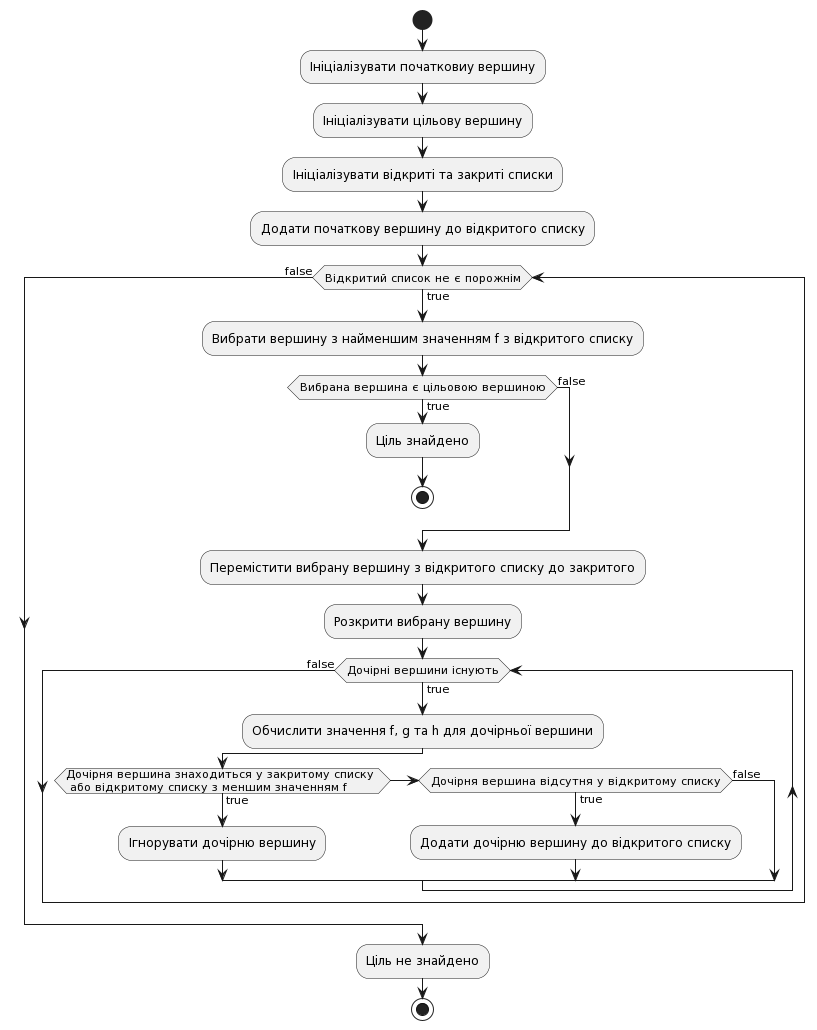
\includegraphics[scale=0.5]{content/chapters/2-implementation-methods/assets/img/a_star_algorithm.png}
    \caption{Блок-схема алгоритму A*}
    \label{fig:a-star}
\end{figure}

Переваги:
\begin{itemize}
    \item Алгоритм A* - це евристичний алгоритм пошуку, який може знайти найкоротший шлях між двома точками більш ефективно, ніж алгоритм Дейкстри.
    \item Евристична функція, що використовується в алгоритмі A*, допомагає спрямовувати пошук до цільової вершини, що може призвести до скорочення часу пошуку.
    \item Алгоритм A* широко використовується в різних додатках, таких як відеоігри, робототехніка та транспорт.
\end{itemize}

Недоліки:
\begin{itemize}
    \item  Точність алгоритму A* сильно залежить від якості евристичної функції, що використовується. Неточна евристична функція може призвести до вибору неоптимальних шляхів.
    \item Може використовувати багато пам'яті, оскільки йому потрібно відстежувати відкриті та закриті множини вершин, відвідані під час пошуку.
    \item У деяких випадках алгоритм A* може не знайти шлях, якщо евристична функція погано спроектована або простір пошуку занадто складний.
\end{itemize}


\subsection{Алгоритм Беллмана-Форда}
\label{subsec:bellman-ford-subsection}

Алгоритм Беллмана-Форда --- це алгоритм найкоротшого шляху з одним джерелом, що означає, що він знаходить найкоротший шлях від однієї вихідної вершини до всіх інших вершин зваженого графа. Він був розроблений Річардом Беллманом і Лестером Фордом у 1950-х роках.

Алгоритм працює, підтримуючи список найкоротших відстаней від вихідної вершини до кожної вершини графа. Спочатку найкоротша відстань до самої вихідної вершини дорівнює 0, а відстань до всіх інших вершин дорівнює нескінченності.

Потім алгоритм ітерує всі ребра графа, послаблюючи їх по черзі. Послаблення ребра означає оновлення найкоротшої відстані до вершини на іншому кінці ребра, якщо знайдено коротший шлях до цієї вершини. Цей процес повторюється V-1 раз, де V - кількість вершин у графі, щоб переконатися, що всі можливі шляхи були досліджені.

Якщо після V-1 ітерацій залишаються ребра, які можна послабити, це означає, що граф містить цикл з від'ємною вагою. Цикл з від'ємною вагою - це цикл ребер у графі, сумарна вага яких від'ємна, і такий цикл може призвести до неправильних результатів роботи алгоритму, оскільки він може призвести до нескінченного циклу зменшення відстаней. Якщо виявлено цикл з від'ємною вагою, алгоритм повідомляє, що граф не містить найкоротших шляхів.

Часова складність алгоритму Беллмана-Форда становить O(V * E), де V - кількість вершин, а E - кількість ребер у графі. Це робить його повільнішим за алгоритм Дейкстри, але він здатен обробляти графи з ребрами з від'ємною вагою, чого не може алгоритм Дейкстри.\\

\begin{figure}[!htp]
    \centering
    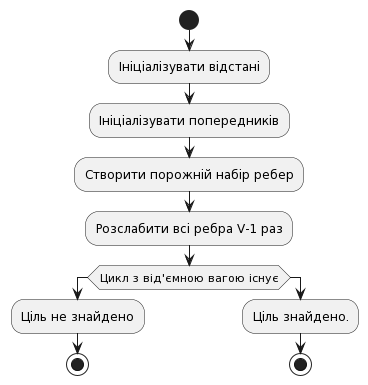
\includegraphics[scale=0.7]{content/chapters/2-implementation-methods/assets/img/bellman-ford_algorithm.png}
    \caption{Блок-схема алгоритму Беллмана-Форда}
    \label{fig:bellman-ford}
\end{figure}

Переваги:
\begin{itemize}
    \item Він може обробляти графи з ребрами з від'ємною вагою, на відміну від алгоритму Дейкстри.
    \item Може виявляти цикли з від'ємною вагою у графі.
    \item Простий у реалізації.
\end{itemize}

Недоліки:
\begin{itemize}
    \item Його часова складність становить O(V * E), що може зробити його повільним для великих графів.
    \item Він не може працювати з графами з циклами від'ємної ваги, оскільки застрягне у нескінченному циклі зменшення відстаней.
\end{itemize}


\subsection{Алгоритм пошуку в ширину}
\label{subsec:bfs-subsection}

Алгоритм пошуку в ширину --- це алгоритм обходу графа, який починається з кореневого вузла і досліджує всі сусідні вузли на поточному рівні глибини, перш ніж перейти на наступний рівень. Це класичний алгоритм, який використовується для обходу графа або деревовидної структури даних.

Алгоритм пошуку в ширину використовує структуру даних у вигляді черги для відстеження вузлів, які потрібно дослідити. Алгоритм починає з додавання кореневого вузла до черги, потім декваліфікує наступний вузол і додає всіх його сусідів до черги. Цей процес продовжується до тих пір, поки не будуть досліджені всі вузли.

Однією з переваг пошуку в ширину є те, що він гарантує найкоротший шлях від кореневої вершини до будь-якої іншої вершини незваженого графа. Це робить його корисним у багатьох додатках, де потрібен найкоротший шлях, наприклад, для пошуку найкоротшого маршруту в дорожній мережі.

Однак пошук в ширину може бути неефективним у графах з великою кількістю ребер, оскільки він повинен дослідити всіх сусідів на кожному рівні, перш ніж перейти на наступний рівень. Це може призвести до додавання великої кількості вузлів до черги, що може спричинити проблеми з пам'яттю.

Таким чином, пошук в ширину - це простий і ефективний алгоритм обходу графа, який корисний у різних додатках, особливо коли потрібно знайти найкоротший шлях. Однак його продуктивність може бути обмежена на великих, складних графах.\\

\begin{figure}[!htp]
    \centering
    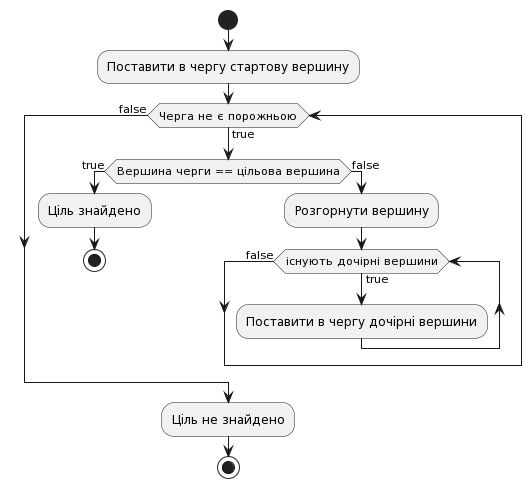
\includegraphics[scale=0.6]{content/chapters/2-implementation-methods/assets/img/bfs_algorithm.png}
    \caption{Блок-схема алгоритму пошуку в ширину}
    \label{fig:bfs}
\end{figure}


Переваги:
\begin{itemize}
    \item Пошук в ширину гарантовано знайде найкоротший шлях до вузла або цілі, якщо вона існує.
    \item Його відносно легко реалізувати і зрозуміти.
    \item Він гарантовано знаходить розв'язок, коли простір пошуку скінченний і коефіцієнт розгалуження скінченний.
    \item Може бути чудовим вибором для додатків, де важливо знайти шлях з найменшою кількістю кроків.
\end{itemize}

Недоліки:
\begin{itemize}
    \item Пошук в ширину може бути повільним і вимагати багато пам'яті, особливо у великих областях пошуку.
    \item Він може витрачати час на дослідження шляхів, які навряд чи приведуть до розв'язку.
    \item Це може бути не найефективніший алгоритм для всіх типів задач, особливо з високим коефіцієнтом розгалуження.
    \item Він може не підходити для задач з нерівномірною вартістю або для задач, де вартість проходження вузла змінюється.
\end{itemize}


\subsection{Вибір алгоритму для вирішення задачі}
\label{subsec:bfs-subsection}


Як видно з розділів вище, існує багато алгоритмів для пошуку найкоротшого маршруту в графі. Для виконання поставленої задачі було обрано алгоритм Дейкстри. Він має кілька переваг, які роблять його гарним вибором для пошуку маршрутів у поставленій задачі.

Однією з головних переваг алгоритму Дейкстри є його простота та ефективність. Це простий алгоритм, який можна легко реалізувати на більшості мов програмування, і він має часову складність O(|E| + |V| log |V|), де |E| - кількість ребер, а |V| - кількість вершин у графі. Це робить його практичним вибором для великих графів з великою кількістю ребер і вершин. На відміну від деяких інших алгоритмів, таких як A* або Беллмана-Форда, він не вимагає евристичної функції або складної структури даних, як черга пріоритетів.

Ще однією перевагою алгоритму Дейкстри є те, що він гарантує знаходження найкоротшого шляху від початкової вершини до всіх інших вершин графа, якщо граф не містить ребер з від'ємною вагою, що для поставленої задачі є неможливим. Ця властивість важлива для багатьох застосувань, таких як маршрутизація в транспортних мережах, де знаходження найкоротшого шляху є важливим для оптимізації часу в дорозі та зменшення витрат.
 
Загалом, алгоритм Дейкстри є надійним та ефективним вибором для пошуку найкоротшого шляху в графі, що робить його популярним для таких додатків, як навігаційні системи та мережева маршрутизація. Простота, ефективність і гарантована оптимальність алгоритму Дейкстри роблять його чудовим вибором для пошуку маршрутів у розроблюваній системі.
